\documentclass[12pt]{article}

\usepackage[total={6.5in,8.75in}, top=2.4cm, left=2.4cm]{geometry}
\usepackage{lineno}
\usepackage{amsmath}
%\usepackage{amssymb}    % used for symbols in figure legends
\usepackage{graphicx}
\usepackage[round,colon,authoryear]{natbib}

\usepackage{bm}
\usepackage{float}
\usepackage{amsmath}
\usepackage{amsfonts}
\usepackage{hyperref}
\usepackage{verbatim}
\usepackage{soul}
\usepackage{color}
\usepackage{setspace}

\bibliographystyle{ecology} % kluwer, plos-natbib, pnas-natbib


\title{Ecological Distance in Spatial Capture-Recapture Models: Supplemental 
files}

\author{
{\bf J. Andrew Royle}\\
USGS Patuxent Wildlife Research Center, Laurel MD \\ \\
{\bf Richard B. Chandler} \\
USGS Patuxent Wildlife Research Center, Laurel MD\\ \\
{\bf Kimberly D. Gazenski} \\
USGS Patuxent Wildlife Research Center, Laurel MD\\ \\
{\bf Tabitha A. Graves} \\
Northern Arizona University, Flagstaff AZ \\ \\
}



\begin{document}

\maketitle

\date

\newpage

\linenumbers


\begin{spacing}{1.2}



\section*{Appendix 1: {\bf R} code for computing least-cost path
  distance and likelihood analysis of the SCR model}


As an example of the cost-weighted distance calculation consider the
following landscape comprised of 16 pixels with unit spacing
identified as follows, along with the pixel-specific cost:
\begin{center}
\begin{verbatim}
  pixel ID                 Cost
 4 8 12 16            100   1   1  1
 3 7 11 15            100 100   1  1
 2 6 10 14            100 100 100  1
 1 5  9 13            100 100   1  1
\end{verbatim}
\end{center}
Then we assigned low cost of 1 to ``good habitat'' pixels (or pixels
we think of as ``highly connected'' by virtue of being in good
habitat) and, conversely, we assign high cost (100) to ``bad
habitat''. So the shortest cost-weighted distance between pixels 5 and
9 in this example is just 1 unit, the shortest cost-distance between
pixels 5 and 10 is $\sqrt{2}(1+1)/2 = 1.414214$ units, the shortest
distance between pixels 4 and 8 is 100 units, while the shortest
cost-distance between 4 and 12 is 150.5. A tough one is: what is the
shortest distance between 7 and 16? An individual at pixel 7 can move
diagonal and pay $sqrt(2)*(100+1)/2 + 1 =72.41778$.  This simple cost
raster is shown in Fig. \ref{ecoldist.fig.raster}.

The {\bf R} commands to create a raster containing the pixel-specific
costs are given as follows for a simple $4\times 4$ raster containing
values either $z=1$ (good habitat) or $z=100$ (bad habitat):
\begin{verbatim}
library(raster)
r<-raster(nrows=4,ncols=4)
projection(r)<- "+proj=utm +zone=12 +datum=WGS84" #sets the projection
#We use UTM here because distances and directions are correct
#i.e., they are adjusted for the earth's curvature
extent(r)<-c(.5,4.5,.5,4.5) #sets the extent of the raster
costs1<- c(100,100,100,100,1,100,100,100,1,1,100,1,1,1,1,1)
values(r)<-matrix(costs1,4,4,byrow=FALSE) #assign the costs to the raster
\end{verbatim}


\begin{figure}
\begin{center}
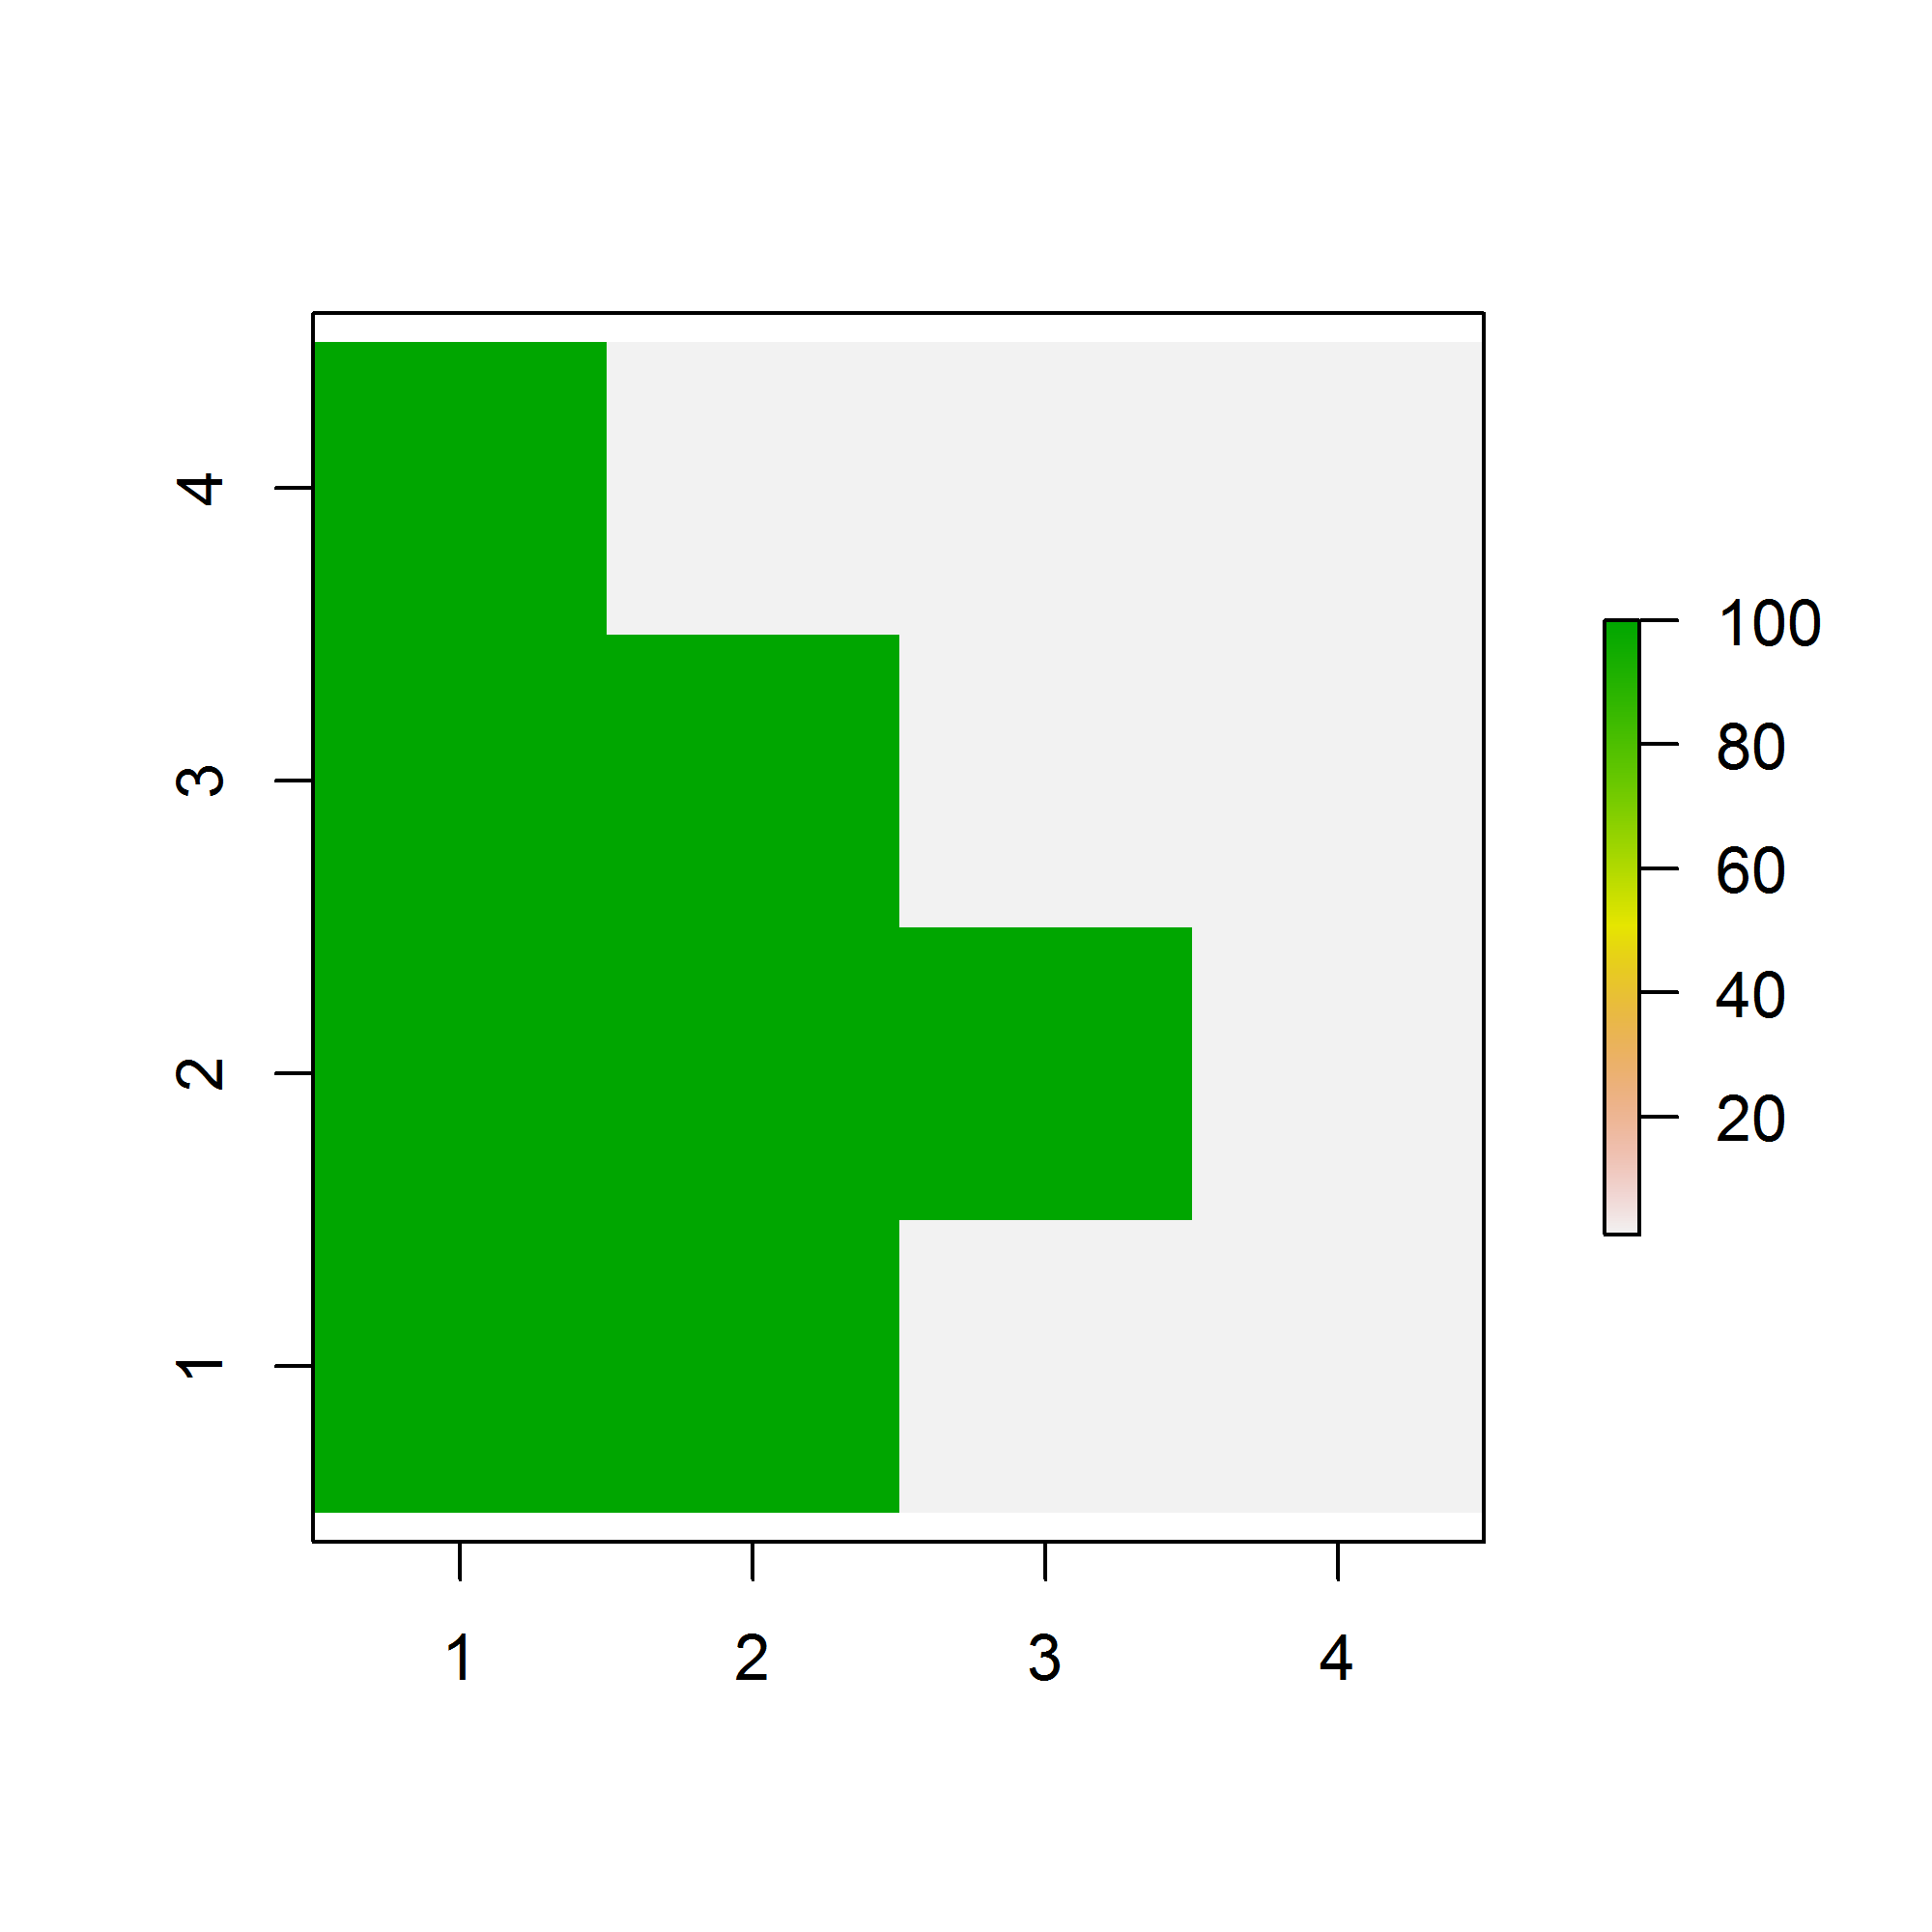
\includegraphics[height=3.25in,width=3.25in]{raster_2values}
\end{center}
\caption{A $4 \times 4$ raster with cost = 1 (white) or 100 (shaded) to represent ease of movement across a pixel.}
\label{ecoldist.fig.raster}
\end{figure}


Once the cost raster is created, the
least-cost path distances are computed with just a couple {\bf R}
commands, and those can be inserted directly into the likelihood
construction for an ordinary spatial capture-recapture model (Appendix
1). The {\bf R} package \mbox{\tt gdistance} uses the implementation
of Dijkstra's algorithm \citep{dijkstra:1959} found in the \mbox{\tt
  igraph} package \citep{csardi:2010}.  Using \mbox{\tt gdistance},
we define the incremental cost of moving from one pixel
to another as the distance-weighted {\it average} of the 2 pixel
costs.

To compute the least-cost path, or the minimum cost-weighted
distances between every pixel and every other pixel, we make use of 
the helper functions \mbox{\tt transition}, which
calculates the cost of moving between neighboring pixels, and
\mbox{\tt geoCorrection} which modifies the costs of moving diagonally
by the additional distance, produce output which feeds into the
function \mbox{\tt costDistance} to compute the pair-wise distance
matrix. For that, we define the center points of each raster.  The
commands altogether are as follows:
\begin{comment}
# The transition function specifies that we'd like to use the mean of
# 2 neighboring pixels as the weight and then takes the inverse to convert
# the costs into conductances, which algorithms within gdistance and
# igraph require. We use the argument directions= 8 to specify that
# all 8 touching pixels are neighbors.)
\end{comment}
\begin{verbatim}
library(gdistance)
tr1<-transition(r,transitionFunction=function(x) 1/mean(x),directions=8)

#The geoCorrection function corrects the conductances for the diagonal neighbors
#and, if the raster is in latitude longitude, also corrects for 
#curvature of the earth's surface

tr1CorrC<-geoCorrection(tr1,type="c",multpl=FALSE,scl=FALSE)

#here we specify the locations that we'd like to calculate distances among
# 
pts<-cbind( sort(rep(1:4,4)),rep(1:4,4))

#the costDistance function calculates the least cost distane among pts using
#the conductances specified in tri1CorrC
costs1<-costDistance(tr1CorrC,pts)
#here we convert costs1 into a matrix
outD<-as.matrix(costs1)
\end{verbatim}



Now we can look at the result and see if it makes sense to us. Here we
print the first 4 columns of this distance matrix and illustrate a
couple of examples of calculating the minimum cost-weighted distance
between points:
\begin{verbatim}
> outD[1:5,1:5]
         1        2        3        4        5
1   0.0000 100.0000 200.0000 205.2426 100.0000
2 100.0000   0.0000 100.0000 200.0000 141.4214
3 200.0000 100.0000   0.0000 100.0000 126.1604
4 205.2426 200.0000 100.0000   0.0000 105.2426
5 100.0000 141.4214 126.1604 105.2426   0.0000
\end{verbatim}

So, to calculate the distance from the first cell in the lower left 
corner to the cell above it, the least cost distance is just the 
mean of the two cells because that is both the shortest line and 
all cells surrounding the first the cost in the first cell is 100 and
the cost in the cell immediately above it is also 100.  So the distance
is (100+100)/2 = 100, which is the same as the mean of the 2 pixels.
%% NOTE: This uses Tabitha's number of pixels
\begin{verbatim}
 plot(r)
 points(pts[1,1],pts[1,2],col="red")
 points(pts[2,1],pts[2,2],col="blue")
 lines(c(1,1),c(1,2))
\end{verbatim}
To move from the pixel in the lower left corner to the upper left corner
points 1 \& 4, the shortest distance is to go directly up.
\begin{verbatim}
 points(pts[4,1],pts[4,2],col="blue")
 lines(c(1,1),c(1,4))
#but the least cost distance is to go around the outside of the high cost area.
 lines(c(1,2),c(1,1)) #with cost = (100 + 100)/2 = 100
 lines(c(2,3),c(1,1)) #with cost = (100 + 1)/2 = 50.5
#To account for the increased distance along the diagonal, we multiply by sqrt(2)
 lines(c(3,4),c(1,2)) #with cost = sqrt(2) * (1+1)/2 = 1.414214
 lines(c(4,3),c(2,3)) #with cost = sqrt(2) * (1+1)/2 = 1.414214
 lines(c(3,2),c(3,4)) #with cost = sqrt(2) * (1+1)/2 = 1.414214
 lines(c(2,1),c(4,4)) #with cost = (100 + 1)/2 = 50.5
 100+50.5* 2+(1.414214)* 3 # = 205.2426 
\end{verbatim}
This matches the distance in our distance matrix between points 1 and 4. 




\section*{Appendix 2: Details for computing the marginal likelihood
  and obtaining the MLEs}


The key operation for computing the likelihood is solving the
2-dimensional integration problem to remove ${\bf s}$. There are some
general purpose {\bf R} packages that implement a number of
multi-dimensional integration routines including 
%\mbox{\tt adapt} \citep{genz_etal:2007} and  %% Not on CRAN anymore
\mbox{\tt R2Cuba} \citep{hahn_etal:2011}.
We won't rely on these extraneous {\bf R} packages but instead will
use perhaps less efficient methods in which we replace the integral
with a summation over an equal area mesh of points on the state-space
${\cal S}$ and explicitly evaluate the integrand at each point. We
invoke the rectangular rule for integration here in which the
integrand is evaluated on a regular grid of points of equal area and
then averaged.  Let $u=1,2,\ldots,nG$ index a grid of $nG$ points,
${\bf s}_{u}$, where the area of grid cell $u$ is constant.  In this
case, the integrand, i.e., the marginal pmf of ${\bf y}_{i}$, is
approximated by

\begin{equation}
         [{\bf y}_{i}|\alpha] = \frac{1}{nG} \sum_{u=1}^{nG}  [ {\bf
            y}_{i} |{\bf s}_u, \alpha]
\label{mle.eq.intlik}
\end{equation}

To deal with the fact that $N$ is unknown, there are two key issues
that need to be addressed.  First is that we don't observe the
``all-zero'' encounter histories (i.e., $y_{ij} = 0$ for all $j$)
corresponding to uncaptured individuals, so we have to make sure we
compute the probability for that all zero encounter history which we
do operationally by tacking a row of zeros onto the encounter history
matrix. We include the number of such all-zero encounter histories as
an unknown parameter of the model, which we label $n_{0}$.  In
addition, we have to be sure to include a combinatorial term to
account for the fact that of the $n$ observed individuals there are
${N \choose n}$ ways to realize a sample of size $n$. The
combinatorial term involves the unknown $n_{0}$ and thus it must be
included in the likelihood.

To compute the integral requires that the bounds of integration are
specified, which is equivalent to prescribing the state-space of the
underlying point process, i.e., ${\cal S}$. Given ${\cal S}$, density
is
computed as $D({\cal S}) = N/||{\cal S}||$. In our simulation study
below we report $N$ as the two are equivalent summaries of the data
set once the state-space is fixed.

We wrote an {\bf R} function to evaluate the likelihood which we optimize
using the {\bf R} function \mbox{\tt optim} (or, alternatively,
\mbox{\tt nlm}).

{\tiny
\begin{verbatim}

### {\bf R} Code
########################################################################
#### Define the likelihood function.
####
	
intlik3ed<-function(start=NULL,y=y,K=NULL,X=traplocs,distmet="ecol",
    covariate,alpha2=NA){  

#start is the starting values for the parameters to be estimated
#y is the data matrix
#K is the number of occasions
#X is the traplocation matrix  with 
#   (one column for x-coords one column for y-coords)
#distmet is either "ecol" or "euclid" for least cost or Euclidean distance

#First, some input checks
if(is.null(K)) return("need sample size")
if(class(covariate)!="RasterLayer") {
 cat("make a raster out of this",fill=TRUE)
 return(NULL)
 }


# Build integration grid. This derives from the covariate raster
# i.e., potential values of s are the mid-point of each raster pixel
nc<-covariate@ncols  #number of columns in the covariate raster
nr<-covariate@nrows  #number of rows in the covariate raster
Xl<-covariate@extent@xmin  #minimum X of the covariate raster
Xu<-covariate@extent@xmax  #maximum X of the covariate raster
Yl<-covariate@extent@ymin  #minimum Y of the covariate raster
Yu<-covariate@extent@ymax  #maximum Y of the covariate raster
SSarea<- (Xu-Xl)*(Yu-Yl)   #Total area of the area over estimating density


###Create potential activity centers evenly distributed across the area
delta<- (Xu-Xl)/nc  #identify offset between locations
xg<-seq(Xl+delta/2,Xu-delta/2,delta) 
yg<-seq(Yl+delta/2,Yu-delta/2,delta) 
npix.x<-length(xg)
npix.y<-length(yg)
area<- (Xu-Xl)*(Yu-Yl)/((npix.x)*(npix.y))  # area of pixels

G<-cbind(rep(xg,npix.y),sort(rep(yg,npix.x)))
nG<-nrow(G) #total number of potential activity centers 
ntraps<- nrow(X)

if(distmet=="euclid")  #if distance metric is Euclidean,
D<- e2dist(X,G)        #calculate distance matrix among traplocs and integration grid

if(distmet=="ecol"){   #if distance metric is Ecological distance 
   if(is.na(alpha2)) alpha2<-exp(start[4]) # if estimating alpha2, use 
                                           #  this starting value
  #the next series of commands calculates the ecological distance matrix 
  cost<- exp(alpha2*covariate)  #create resistance surface
  #find neighbors and calculate conductances among neighbors
  tr1<-transition(cost,transitionFunction=function(x) 1/mean(x),directions=8)
  tr1CorrC<-geoCorrection(tr1,type="c",multpl=FALSE,scl=FALSE) #adjust diag.conductances
  D<-costDistance(tr1CorrC,X,G)  #calculate the ecological distance matrix
  }

if(is.null(start)) start<-c(0,0,0,0) #if no starting values were given, assign as 0s
alpha0<-start[1]
alpha1<-start[2]
n0<-exp(start[3])

#calculate the capture probability at each trap location for each potential 
#activity center, equivalent to each location in the integration grid

probcap<- (exp(alpha0)/(1+exp(alpha0)))*exp(-alpha1*D*D) 

#create integrand matrix (# traplocations X #potential activity centers)

Pm<-matrix(NA,nrow=ntraps,ncol=nG) 
ymat<-y

#Add a zero capture record to the capture history. 
#We weight this last record later to get the total
#estimated number of individuals

ymat<-rbind(y,rep(0,ncol(y)))  
lik.marg<-rep(NA,nrow(ymat)) #create vector to store the marginal likelihood

#calculate the likelihood  
#loop through each individual (plus the all zero-capture record) in capture history

for(i in 1:nrow(ymat)){ 
#calculate the probability of capturing individual i the recorded #of times 
#in each trap (rows) when there are K occasions 
#at each potential activity center (columns).
#These are logged for numerical stability (so very small probabilities recorded)

Pm[1:length(Pm)]<- (dbinom(rep(ymat[i,],nG),rep(K,nG),probcap[1:length(Pm)],log=TRUE))

#conditional on s likelihood (for individual i for each potential activity center)
#exponentiate to remove log above now that the numbers are larger

lik.cond<- exp(colSums(Pm,na.rm=TRUE) )

#the marginal likelihood is formed by explicitly evaluating the integrand 
#on our integration grid, averaging over the conditional likelihood 
#at all potential activity centers as described above
lik.marg[i]<- sum( lik.cond*(1/nG) )  
}      

#define weights = 1 for all individuals we captured, 
#and estimate weight for the number of individuals that were not captured =n0                 
                     
nv<-c(rep(1,length(lik.marg)-1),n0)  
#calculate combinatorial term to account for (N choose n) ways to  
#realize sample of size n
part1<- lgamma(nrow(y)+n0+1) - lgamma(n0+1) #combinatorial term  

###Multiply by weight vector(nv) and sum resulting marginal likelihoods for all individuals
part2<- sum(nv*log(lik.marg))  
out<-  -1*(part1+ part2)  #final negative log likelihood
attr(out,"SSarea")<- SSarea   #save an attribute that has just the
                              #  area of the integration grid
out   # the value of the neg log likelihood
}
\end{verbatim}
}



\newpage

\section*{Appendix 3: {\bf R} Code for simulation study }

{\tiny
\begin{verbatim}

### We require 3 R libraries
library("shapefiles")
library("gdistance")
library("raster")

###Before we get started, we'll run some utility functions 
## UTILITY FUNCTIONS 
## 
## PUT ALL OF THE OBJECTS BELOW INTO YOUR WORKSPACE
##

####This function creates a color scale used with the function image
image.scale <-
function (z, col, x, y = NULL, size = NULL, digits = 2, labels = c("breaks", 
    "ranges"))
{
    # sort out the location
    n <- length(col)
    usr <- par("usr")
    mx <- mean(usr[1:2]); my <- mean(usr[3:4])
    dx <- diff(usr[1:2]); dy <- diff(usr[3:4])
    if (missing(x))
        x <- mx + 1.05*dx/2	# default x to right of image
    else if (is.list(x)) {
        if (length(x$x) == 2) 
          size <- c(diff(x$x), -diff(x$y)/n)
        y <- x$y[1]
        x <- x$x[1]
    } else x <- x[1]
    if (is.null(size))
        if (is.null(y)) {
          size <- 0.618*dy/n	# default size, golden ratio
          y <- my + 0.618*dy/2	# default y to give centred scale
        } else size <- (y-my)*2/n
    if (length(size)==1)
        size <- rep(size, 2)	# default square boxes
    if (is.null(y))
        y <- my + n*size[2]/2
    # draw the image scale
    i <- seq(along = col)
    rect(x, y - i * size[2], x + size[1], y - (i - 1) * size[2], 
        col = rev(col), xpd = TRUE)
    # sort out the labels
    rng <- range(z, na.rm = TRUE)
    bks <- seq(from = rng[2], to = rng[1], length = n + 1)
    bks <- formatC(bks, format="f", digits=digits)
    labels <- match.arg(labels)
    if (labels == "breaks")
        ypts <- y - c(0, i) * size[2]
    else {
        bks <- paste(bks[-1], bks[-(n+1)], sep = " - ")
        ypts <- y - (i - 0.5) * size[2]
    }
    text(x = x + 1.2 * size[1], y = ypts, labels = bks, adj =
        ifelse(size[1]>0, 0, 1), xpd = TRUE) 
}

####This function makes a nice 3D plot
spatial.plot <-
function(x,y,add=TRUE,cx=1){
 nc<-as.numeric(cut(y,20))
if(!add) plot(x,pch=" ")
 points(x,pch=20,col=terrain.colors(20)[nc],cex=cx)
image.scale(y,col=terrain.colors(20))
}

####This function calculates geographic distances among two sets of locations 
####e.g., will work for traplocs and integration grid instead of just among traplocs 
e2dist <- function (x, y) {
    i <- sort(rep(1:nrow(y), nrow(x)))
    dvec <- sqrt((x[, 1] - y[i, 1])^2 + (x[, 2] - y[i, 2])^2)
    matrix(dvec, nrow = nrow(x), ncol = nrow(y), byrow = F)
    }
####This function calculates summary statistics for an input x
smy.fn <- function(x){
    c(mean(x),sqrt(var(x)),quantile(x,c(0.025,0.50,0.975)))
    }

##########################################################################
####CREATE COVARIATES
### Now we create the covariates that we will use in the simulation.
### The following block of code creates a "patchy" looking covariate to use
### in our cost function. It uses a standard method for generating a correlated
### multivariate normal vector of length, in this case, 400 (one value for each
### pixel). One can use any correlation function here but we chose a standard
### exponential model with range parameter 0.5.
par(mfrow=c(1,1))
#setting the seed ensures that your results will match ours 
#delete this line for stochastic results
set.seed(12)  

n.pix= 20 #number of pixels in raster
r<-raster(nrows=n.pix,ncols=n.pix) #create an empty raster
projection(r)<- "+proj=utm +zone=12 +datum=WGS84" #set the projection to be UTMs
xmin<- ymin<- .5
xmax<- ymax<- 4.5
extent(r)<-c(xmin,xmax,ymin,ymax) #set the extent of the raster
delta<- (xmax-xmin)/n.pix  #find the distance between points 
gx<- seq(xmin + delta/2, xmax-delta/2,,n.pix) #create a sequence for the x locations
gy<- rev(gx) #create a sequence for the y locations in reverse order
gx<-sort(rep(gx,20)) #sort and repeat the sequence of x locations for all columns
gy<-rep(gy,20) #repeat the y locations for all rows
grid<-cbind(gx,gy) #bind the x and y components of the locations
Dmat<-as.matrix(dist(grid)) #calculate the Euclidean distances among the potential activity centers 
V<-exp(-Dmat/.5)  #Create the correlation function: standard exponential with range paramater 0.5
z<-t(chol(V))%*%rnorm(400) #Create the correlated variable z, with some random noise
z<- (z-mean(z))/sqrt(var(as.vector(z))) #center the correlated variable
values(r)<-matrix(z,20,20,byrow=FALSE)  #assign z to the raster r
#plot the covariate
par(mfrow=c(2,1)) 
hist(z)
plot(r)
points(grid)
#dev.off() #removes figure
covariate.patchy<- z*sqrt(1.68) + .168   #approx. same scale as systematic covariate below
values(r)<-matrix(covariate.patchy,20,20,byrow=FALSE) #assign the scaled covariate values to r
covariate.patchy<- r  #create a new raster called covariate.patchy
#class(covariate.patchy) #check to confirm that covariate.patchy is a RasterLayer

## SYSTEMATIC COVARIATE
## It's much simpler to build a systematic (or trend) covariate.
## Here we defined as a trend from NW to SE
## 
cost<-matrix(NA,nrow=n.pix,ncol=n.pix)
cost<-row(cost)+col(cost)
covariate.trend<- (cost-20)/10 #define cost values
values(r)<-matrix(covariate.trend,n.pix,n.pix,byrow=FALSE) #assign costs to raster r
covariate.trend<-r
class(covariate.trend)
plot(covariate.trend)


####SIMULATION FUNCTION
####Next we define a few conditions and then the simulation function, 
####where we simulate activity centers and trap locations, calculate
####the probability of capture, simulate captures, and then fit the 
####simulated data.  To do this a single time, first run the utility
####functions below, run the following conditions, and then run only 
####the code inside of the function.

N<-200  #the number of individuals=activity centers
alpha0<- -2  
sigma<- .5  #scale parameter for the distance distribution
K<- 5
nsim=1
covariate<-covariate.patchy

sim.fn<-function(N=200,nsim=100,alpha0= -2, sigma=.5, K=5,covariate){
#N= true number of individuals
#nsim = the number of simulations you'd like to run
#alpha0 is the resistance covariate
#sigma is the scale parameter
#K is the number of occasions
#covariate refers to the RasterLayer object that is the covariate

cl<-match.call() #stores all the arguments in the function call for later reference
#Create matrices to store the output
simout2<-simout1<-simout3<-matrix(NA,nrow=nsim,ncol=5)
alpha1<- 1/(2*sigma*sigma) #calculate alpha based on the sigma (scale parameter)

#Create a raster object
r<-raster(nrows=20,ncols=20)
projection(r)<- "+proj=utm +zone=12 +datum=WGS84" #assign the projection
extent(r)<-c(.5,4.5,.5,4.5)  #assign the extent of the raster
alpha2<-1 #assign the resistance coefficient
cost<- exp(alpha2*covariate) #calculate the resistance surface 
#(i.e. the cost per pixel for each pixel of the covariate

#par(mfrow=c(1,1))
#plot(r)
r<-cost #rename the cost raster r
#identify neighbors and calculate distances as conductances (1/average distance between 2 pixels)
tr1<-transition(r,transitionFunction=function(x) 1/mean(x),directions=8)
#correct the diagonal distances 
tr1CorrC<-geoCorrection(tr1,type="c",multpl=FALSE,scl=FALSE) 

#Create the trap locations composed of locations xg, yg
xg<-seq(1,4,1)
yg<-4:1
traplocs<-cbind( sort(rep(xg,4)),rep(yg,4))
#graph the traplocations
points(traplocs,pch=20,col="red")
ntraps<-nrow(traplocs)


for(sim in 1:nsim){

#Create the activity centers, distributed uniformly in the state space= extent
#Note that the raster defines the state space because least cost distance 
#can not be calculated where there are no covariate values.

S<-cbind(runif(N,.5,4.5),runif(N,.5,4.5))

#calculate the least cost distances between activity centers and traplocations 

D<- costDistance(tr1CorrC,S,traplocs)  #N x ntraps matrix

#calculate the probability of capture based on the weighted distance distribution

probcap<-plogis(alpha0)*exp(-alpha1*D*D) #N X ntraps matrix

# now generate the number of encounters of every individual in every trap

Y<-matrix(NA,nrow=N,ncol=ntraps) #N X ntraps matrix
for(i in 1:nrow(Y)){
 Y[i,]<-rbinom(ntraps,K,probcap[i,]) #simulate # of encounters from K occasions
}

#select only those individuals that were counted at least once for the capture history

Y<-Y[apply(Y,1,sum)>0,] #matrix of N actually captured X ntraps
n0<- N-nrow(Y)  #number of zero-encounter histories

#calculate the likelihood based solely on Euclidean distance
frog<-optim(c(alpha0,alpha1,log(n0)),intlik3ed,hessian=TRUE,y=Y,K=K,X=traplocs,
               distmet="euclid",covariate=covariate,alpha2=1)
# if using nlm and sometimes with optim, warnings can be produced. This
# is due to parameters outside of parameter space or small number 
# arithmetic. 
# ignore these warnings.

simout1[sim,]<-c(frog$par,NA,nrow(Y))

#calculate the likelihood based on ecological distance with cost coefficient fixed
frog<-optim(c(alpha0,alpha1,log(n0)),intlik3ed,hessian=TRUE,y=Y,K=K,X=traplocs,
               distmet="ecol",covariate=covariate,alpha2=1)
simout2[sim,]<-c(frog$par,NA,nrow(Y))

#calculate the likelihood based on ecological distance with cost coefficient estimated
frog<-optim(c(alpha0,alpha1,log(n0),-.3),intlik3ed,hessian=TRUE,y=Y,K=K,X=traplocs,
               distmet="ecol",covariate=covariate,alpha2=NA)
simout3[sim,]<-c(frog$par,nrow(Y))
}
#output results of simulations, plus the inputs to the function (cl defined above) 
list(simout1=simout1,simout2=simout2,simout3=simout3,call=cl)

}  #end of the simulation function



#####The next groups of code were used to specify and summarize the simulations reported in the paper.
###
### R commands to carry-out the simulations. MUST SOURCE likelihood function first -- SEE BELOW
### This takes 1-2 days to run for nsims=100
###
###

nsims<-50
###
####Systematic covariate 
###
simout.low.N100<-sim.fn(N=100,nsim=nsims,alpha0=-2,sigma=.5,K=5,covariate=covariate.trend)
simout.low.N200<-sim.fn(N=200,nsim=nsims,alpha0= -2, sigma=.5,K=5,covariate=covariate.trend)
simout.reallylow.N100<-sim.fn(N=100,nsim=nsims,alpha0=-2,sigma=.5,K=3,covariate=covariate.trend)
simout.reallylow.N200<-sim.fn(N=200,nsim=nsims,alpha0= -2, sigma=.5,K=3,covariate=covariate.trend)
simout.high.N100<-sim.fn(N=100,nsim=nsims,alpha0=-2,sigma=.5,K=10,covariate=covariate.trend)
simout.high.N200<-sim.fn(N=200,nsim=nsims,alpha0= -2, sigma=.5,K=10,covariate=covariate.trend)
###
### R commands to summarize the simulation output
###
mat<-matrix(NA,nrow=9,ncol=10)
for(i in 1:3){
mat[i,1:5]<- smy.fn(exp(simout.reallylow.N100[[i]][,3]) + simout.reallylow.N100[[i]][,5])
mat[i,6:10]<- smy.fn(exp(simout.reallylow.N200[[i]][,3]) + simout.reallylow.N200[[i]][,5])
mat[3+i,1:5]<- smy.fn(exp(simout.low.N100[[i]][,3]) + simout.low.N100[[i]][,5])
mat[3+i,6:10]<- smy.fn(exp(simout.low.N200[[i]][,3]) + simout.low.N200[[i]][,5])
mat[6+i,1:5]<- smy.fn(exp(simout.high.N100[[i]][,3]) + simout.high.N100[[i]][,5])
mat[6+i,6:10]<- smy.fn(exp(simout.high.N200[[i]][,3]) + simout.high.N200[[i]][,5])
}

### 
#### Patchy covariate
###
simout.low.N100.k<-sim.fn(N=100,nsim=nsims,alpha0=-2,sigma=.5,K=5,covariate=covariate.patchy)
simout.low.N200.k<-sim.fn(N=200,nsim=nsims,alpha0= -2, sigma=.5,K=5,covariate=covariate.patchy)
simout.reallylow.N100.k<-sim.fn(N=100,nsim=nsims,alpha0=-2,sigma=.5,K=3,covariate=covariate.patchy)
simout.reallylow.N200.k<-sim.fn(N=200,nsim=nsims,alpha0= -2, sigma=.5,K=3,covariate=covariate.patchy)
simout.high.N100.k<-sim.fn(N=100,nsim=nsims,alpha0=-2,sigma=.5,K=10,covariate=covariate.patchy)
simout.high.N200.k<-sim.fn(N=200,nsim=nsims,alpha0= -2, sigma=.5,K=10,covariate=covariate.patchy)
###
### R commands to summarize the simulation output
###
mat.k<-matrix(NA,nrow=9,ncol=10)
for(i in 1:3){
mat.k[i,1:5]<- smy.fn(exp(simout.reallylow.N100.k[[i]][,3]) + simout.reallylow.N100.k[[i]][,5])
mat.k[i,6:10]<- smy.fn(exp(simout.reallylow.N200.k[[i]][,3]) + simout.reallylow.N200.k[[i]][,5])
mat.k[3+i,1:5]<- smy.fn(exp(simout.low.N100.k[[i]][,3]) + simout.low.N100.k[[i]][,5])
mat.k[3+i,6:10]<- smy.fn(exp(simout.low.N200.k[[i]][,3]) + simout.low.N200.k[[i]][,5])
mat.k[6+i,1:5]<- smy.fn(exp(simout.high.N100.k[[i]][,3]) + simout.high.N100.k[[i]][,5])
mat.k[6+i,6:10]<- smy.fn(exp(simout.high.N200.k[[i]][,3]) + simout.high.N200.k[[i]][,5])
}



\end{verbatim}
}

\newpage

\section*{Appendix 4:  MLE summary statistics for reanalysis of the
  systematic landscape}


For both landscapes and all simulation conditions (levels of $K$ and
$N$) the average sample sizes of individuals captured are given in
Table~\ref{tab.samplesize}.  


\begin{table}
\centering
\caption{
Expected sample sizes of captured individuals under each configuration of
$N$ (population size for the prescribed state-space) and $K$ (number of replicate samples).
}
\begin{tabular}{l|rrrr}
 & \multicolumn{2}{c}{Systematic} & \multicolumn{2}{c}{Patchy}  \\
    & N=100 &  N=200  &   N=100 &  N=200  \\ \hline
K=3 &  38.69 &   78.17  &   37.30 &   74.93  \\
K=5 &  51.10 &  103.18  &   51.89 &  103.71 \\
K=10&  65.81 &  132.39  &   69.44 &  138.76 \\
\end{tabular}
\label{tab.samplesize}
\end{table}



\begin{table}
{\small
\caption{Simulation results for estimating population size $N$ for a prescribed state-space with
$N=100$ or $N=200$ and various levels of replication ($K$) chosen to affect the observed sample
size of individuals. These results correspond to those of the
systematic landscape in Table 2 except with the traps
moved 0.5 units in from the boundary of the raster.
Each grouping of 3 rows (for a given value of $K$) summarizes the
performance of $\hat{N}$ under 3 distance models: (1) A model in which
Euclidean distance was used (``euclid''); (2) A model in which the
least-cost path distance was used, with the coefficient of the cost
function fixed (``lcp/known''); and (3) A model in which the
coefficient was estimated (``lcp/est''). The summary statistics of the
sampling distribution reported are the mean, standard deviation
(``SD'') and quantiles (0.025, 0.50, 0.975).
}
{\bf Systematic trend raster:} \\
\begin{tabular}{l|rrrrr|rrrrr}
         & \multicolumn{5}{c}{N=100   } & \multicolumn{5}{c}{N=200  }  \\
         &   mean &  SD  & 0.025 & 0.50 & 0.975  & mean  & SD   & 0.025 & 0.50  & 0.975 \\ \hline
K=3      &        &      &       &      &        &       &      &       &       &       \\
euclid   &   84.48& 20.42& 51.16 & 81.51& 140.62 &163.70 &24.55 &126.64 &157.67 &223.63 \\
lcp/known&  104.14& 25.49& 65.67 &101.50& 173.19 &200.16 &29.27 &158.65 &191.04 &268.78\\
lcp/est  &  105.90& 26.19& 65.95 &103.40& 182.30 &201.34 &29.54 &161.88 &192.36 &268.98\\
K=5      &        &      &       &      &        &       &      &       &       &       \\
euclid   & 81.21  &11.33 &61.35  &79.20 & 98.86  &163.27 &13.06 &140.21 &162.97 &185.94\\
lcp/known& 99.93  &12.86 &76.97  &99.75 &117.76  &199.80 &16.60 &170.25 &198.23 &227.66\\
lcp/est  & 100.84 &13.15 &79.96  &99.51 &119.08  &200.25 &16.53 &168.88 &199.29 &227.39\\
K=10     &        &      &       &      &        &       &      &       &       &       \\
euclid   &  80.10 & 7.81 &66.45  &79.14 &93.33   &158.40 & 9.25 &142.74 &157.86 &173.18\\
lcp/known& 100.07 & 9.50 &82.99  &100.33&114.81  &197.62 &12.58 &171.95 &199.21 &217.19\\
lcp/est  & 100.10 & 9.88 &82.31  &100.91&116.27  &197.52 &13.03 &169.49 &200.68 &217.82\\ \hline
\end{tabular}
}
\label{tab.results3}
\end{table}






\begin{table}
\centering
\caption{
Mean of sampling distribution of the cost function parameter
$\alpha_{2}$ for the different simulation
conditions.  The simulation for the systematic landscape was repeated
with sample locations concentrated away from the boundary of the
landscape to avoid truncation bias in computing the integrated
likelihood. Results for that case are shown in rows 4-6.
}
\begin{tabular}{l|rrrr}
 & \multicolumn{2}{c}{Patchy} & \multicolumn{2}{c}{Systematic} \\
    & N=100 &  N=200  &   N=100 &  N=200  \\ \hline
K=3 &   1.05&    1.03 &     1.17 & 1.14 \\
K=5 &   1.02&    1.01 &     1.12 &1.12 \\
K=10&   1.01&    1.00 &     1.10 &1.08 \\ \hline
K=3    &       &         &     1.08 & 1.04 \\
K=5    &       &         &     1.02 & 1.02 \\
K=10    &       &         &     1.01 & 1.01 \\
\end{tabular}
\label{tab.results2}
\end{table}






\newpage


\bibliography{EDmanuscript-supplements-v3.bbl}


\end{spacing}

\end{document}






